\documentclass[9pt, twocolumn]{extarticle}
% \documentclass[9pt, onecolumn]{extarticle}

%%% Using extarticle instead of the standard article class to allow 8pt font size
%%% Title and author fields are manually resized (e.g., \Huge, \large) for better fitting
%%% \vspace*{-\topskip} is applied in \maketitle to remove the extra top margin above the title

\usepackage{graphicx}
\graphicspath{{figs/}}
\usepackage[a4paper, margin=1.5cm, bottom=2.5cm]{geometry}
\usepackage{float}
\usepackage{subfig}
\usepackage{caption}
\usepackage{tabularx}
\usepackage{booktabs}
\usepackage[utf8]{inputenc}
\usepackage[T1]{fontenc}
\usepackage{longtable}
% \usepackage{stfloats}  % Commented out - package not available
\usepackage{amsmath}
\usepackage{amssymb}
\usepackage{titlesec}
\usepackage{setspace}
\usepackage{xcolor}
\definecolor{UofT_blue}{HTML}{0baedd}
\usepackage[colorlinks=true,
            linkcolor=UofT_blue,
            urlcolor=UofT_blue,
            citecolor=UofT_blue]{hyperref}
\usepackage[
  backend=biber,
  style=numeric,          % numbered refs
  citestyle=numeric-comp, % [1-3] compression
  sorting=none            % order of citation
  ]{biblatex}
  \addbibresource{references.bib}

\newcommand{\mystretch}{1.2}
\newcommand{\myfigmargin}{4pt}


\setlength{\textfloatsep}{\myfigmargin}    % text ↔ top/bottom floats
\setlength{\intextsep}{\myfigmargin}       % text ↔ here-placed floats ([h])
\setlength{\floatsep}{\myfigmargin}        % between floats
\setlength{\dbltextfloatsep}{\myfigmargin} % two-column floats (figure*)
\setlength{\dblfloatsep}{\myfigmargin}


\captionsetup[figure]{belowskip=0pt, skip=4pt, labelfont=bf, justification=justified, singlelinecheck=false, font={stretch=\mystretch}}
\captionsetup[subfloat]{labelfont=normalfont, justification=centering, singlelinecheck=false, farskip=4pt,captionskip=0pt, font={stretch=\mystretch}}
\captionsetup[subfloat]{belowskip=-14pt, font={stretch=\mystretch}}
\captionsetup[table]{labelfont=bf, justification=justified, singlelinecheck=false, skip=2pt, farskip=0pt, captionskip=0pt, belowskip=0pt, font={stretch=\mystretch}}
  
\renewcommand{\baselinestretch}{\mystretch} % 1.2x line spacing
  
\setlength{\columnsep}{0.5cm}
  
\makeatletter
\renewcommand\section{\@startsection{section}{1}{0pt}%
  {0.8ex plus 0.5ex minus 0.2ex}%
  {0.5ex}%
  {\normalfont\Large\bfseries}}
\makeatother


\makeatletter
\renewcommand{\maketitle}{\bgroup\setlength{\parindent}{0pt}
\vspace*{-\topskip}% remove the top margin above title
\begin{flushleft}
  \huge\textbf{\@title}

  \vspace{0.20cm}

  \normalsize\@author \hfill \normalsize\@date

  \vspace{0.25cm}\hrule\vspace{0.25cm}
\end{flushleft}
\egroup}
\makeatother


\begin{document}

% Cover Page
\begin{titlepage}
\centering
\vspace*{1.5cm}

% Title
{\fontsize{36}{42}\selectfont\bfseries\color{UofT_blue} Basin-Scale Hydrologic Characterization of the\\La Dore Basin\par}
\vspace{3.5cm}

% Author
{\fontsize{18}{18}\selectfont Ali Haghighi\par}
\vspace{2cm}

% Advisors
{\fontsize{18}{18}\selectfont Surface Water Hydrology\par}
{\fontsize{18}{24}\selectfont Dr. Afshin Ashrafzadeh\par}
\vspace{3cm}

% Date
{\fontsize{14}{14}\selectfont\today\par}
\vspace{1.5cm}

% Logos
\begin{figure}[h]
\centering
% keep horizontal spacing even if the second logo is disabled
\hspace*{0.5cm}
\includegraphics[height=3.5cm]{figs/U of T Logo.pdf}
\hspace*{0.5cm}
% \includegraphics[height=2cm]{figs/Universite de Strasbourg Logo.pdf} % (disabled for now)
\end{figure}

\vfill

\end{titlepage}

\newpage

\section*{Abstract}

This report was prepared for the Master's Surface Hydrology course taught by Dr.\ Afshin Ashrafzadeh (Fall 2025). The analysis is based on CAMELS-FR, a catchment-scale hydrologic dataset for France that provides standardized basin attributes, meteorological forcings, and discharge time series; from CAMELS-FR, the La Dore basin at Saint-Gervais-sous-Meymont (station code K287191001; area 795\,km²) was selected as a case study. We characterize basin physiography (morphometry, stream network, hypsometry), hydroclimate and runoff behavior (daily and monthly precipitation, discharge, and potential evapotranspiration; flow duration curve), and the long-term water balance for 1990--2020. Mean annual precipitation is about 1055\,mm/yr, runoff 381\,mm/yr, and the runoff ratio is 0.36. The project codebase is available at \href{https://github.com/Alioax/hydro}{github.com/Alioax/hydro}; the codebase includes hooks for remote-sensing products (GPM IMERG, SMAP) to support future extensions, and a planned end-of-report discussion will outline possible research directions building on this workflow.

% ========== 1) INTRODUCTION ==========
\section{Introduction}

Basin-scale hydrologic characterization provides essential context for water-resources assessment, flood and low-flow analysis, and interpretation of runoff-generation processes. Using standardized datasets and a consistent workflow makes it possible to compare catchments objectively, communicate key hydrologic signatures, and establish a baseline for subsequent model development or the integration of remote-sensing products. This report builds on the CAMELS-FR dataset \cite{WH7FJR_2024,Delaigue2025CAMELSFR}.

In this report, the project includes:
\begin{itemize}\setlength\itemsep{0.1em}\setlength\parskip{0pt}\setlength\topsep{0.1em}
  \item Basin physiography and drainage structure (morphometry, stream network, hypsometry).
  \item Hydroclimate and runoff behavior from CAMELS-FR time series.
  \item Water balance (annual and seasonal): precipitation, runoff, PET, residual.
\end{itemize}

\textbf{Study scope.} This report uses the CAMELS-FR dataset and SRTM DEM for one focus basin (La Dore, station K287191001). IMERG and SMAP remote-sensing products are not used in the present analysis; they are reserved for future work.

% ========== 2) STUDY AREA ==========
\section{Study Area}

\subsection{Location and Boundary}
\label{sec:location}

The study basin is La Dore at Saint-Gervais-sous-Meymont (station code K287191001), with a catchment area of 795\,km² and an outlet elevation of 398\,m\,a.s.l. The outlet gauge (monitoring station) is located roughly 100\,km west of the city of Lyon. Figure~\ref{fig:basin_map} shows the catchment boundary and gauge outlet on a basemap.

\begin{figure}[!htbp]
\centering
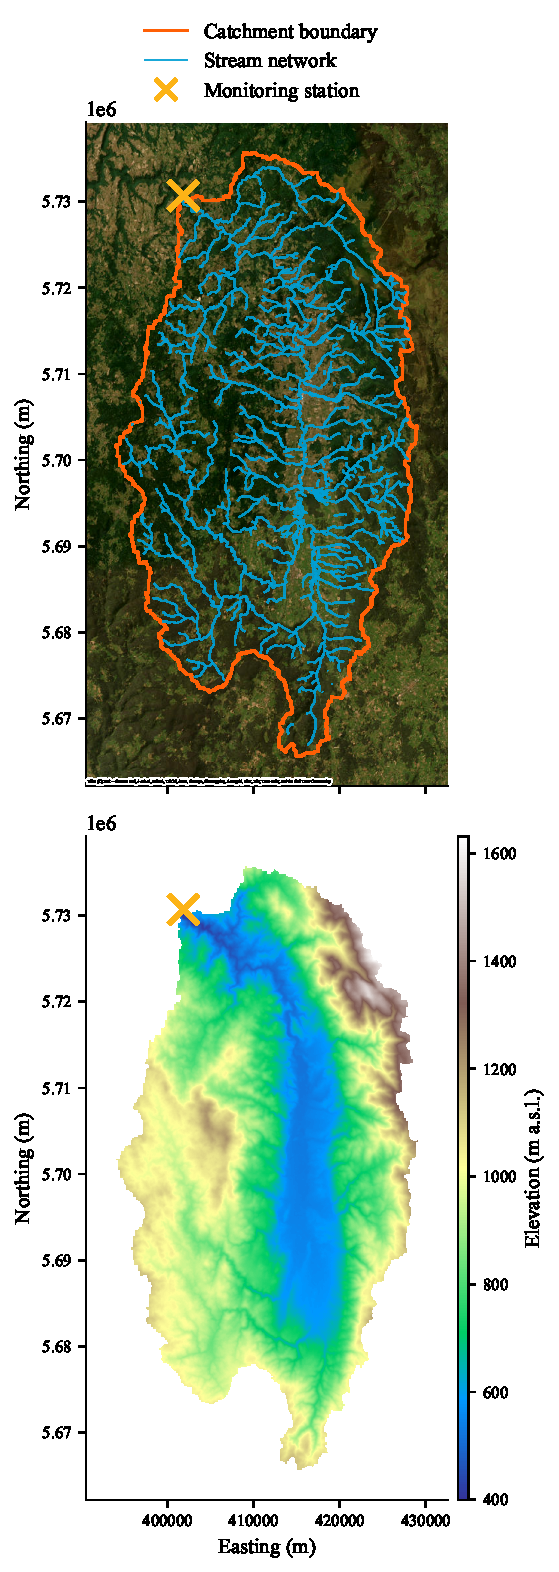
\includegraphics[width=0.95\columnwidth]{map_basin_outlet}
\caption{Catchment boundary and gauge outlet for station K287191001 (La Dore à Saint-Gervais-sous-Meymont). Area 795\,km²; outlet elevation 398\,m\,a.s.l. The stream network displayed is from an OpenStreetMap-derived stream product. Map displayed in Web Mercator (EPSG:3857).}
\label{fig:basin_map}
\end{figure}

The basin lies in the Massif Central (France); coordinates at the outlet are approximately 3.61°E, 45.69°N (WGS84). It is one of the CAMELS-FR basins with area 500--1000\,km² (see Appendix~\ref{app:basins}). The climate is temperate oceanic with continental influence; precipitation and runoff exhibit marked seasonality (winter--spring high flows, summer low flows).

% ========== 3) DATA SOURCES ==========
\section{Data Sources}

\subsection{CAMELS-FR}

This project uses the CAMELS-FR large-sample hydrology dataset for France \cite{WH7FJR_2024, Delaigue2025CAMELSFR}. CAMELS-FR provides catchment boundaries and gauge locations, standardized catchment attributes (e.g., basin area, elevation and relief, slopes, drainage-network and shape indices), and hydro-meteorological time series including precipitation, air temperature, potential evapotranspiration, and discharge.

In this report, CAMELS-FR is used to (a) define the study basin and its boundary/outlet, (b) extract basin physiographic descriptors for the morphometric summary, and (c) supply the daily/monthly time series used for hydroclimate characterization, the flow-duration curve, and the 1990--2020 water-balance analysis. CAMELS-FR also provides a companion set of standardized graphical fact sheets for each basin; see Appendix~\ref{app:fact_sheet} for the fact sheet for La Dore and an at-a-glance summary with additional basin details.

\subsection{Terrain Data (SRTM DEM)}

SRTM DEM (30\,m) is used to derive terrain, drainage structure, and elevation--area relationships. GPM IMERG \cite{imergdp} and SMAP \cite{smap} are available for future extension (precipitation bias, soil moisture) but are not used in this report.

\subsection{Analysis Period and Data Screening}

Unless stated otherwise, the analysis period is 1990--2020 for the water balance and flow-duration curve, while the time-series snippet uses 2017--2020. Days with missing or invalid discharge are dropped; monthly aggregates use only months with at least 90\% valid days.

% ========== 4) EXPLORATORY ANALYSES ==========
\section{Exploratory Analyses}

This class project is organized as a set of exploratory analyses. For each analysis, we briefly summarize the workflow and then report the key outputs.

\subsection{Basin Physiography and Drainage Structure}

\textbf{Workflow.} Basin boundary and outlet are taken from CAMELS-FR geography (catchment boundaries and gauge outlet \texttt{.gpkg}). Basin terrain metrics and hypsometry are derived from SRTM DEM.

The stream network shown in Figure~\ref{fig:basin_map} is taken from an OpenStreetMap-derived stream product (not delineated in this project). We attempted to delineate streams from the DEM using \texttt{pysheds} \cite{bartos_2020} with D8 flow direction and flow accumulation; however, the extracted network and main channel were not satisfactory despite extensive debugging. As a result, we used the existing stream product for visualization. A priority for future work is to diagnose and fix the DEM-based delineation (e.g., preprocessing, sinks/breaching, burn-in, projection/resolution consistency, and threshold selection) so the stream network can be generated reproducibly from the DEM.

\textbf{Outputs.} Figure~\ref{fig:basin_map} provides a plan-view overview (boundary, drainage, and outlet gauge). Table~\ref{tab:basin_metrics} summarizes basin geometry, elevation, slope, shape, and drainage metrics.

\begin{table}[htbp]
\centering
\caption{Basin physiography and morphometric metrics for La Dore (K287191001).}
\label{tab:basin_metrics}
\begin{tabular}{ll}
\toprule
Metric & Value \\
\midrule
Area (km²) & 795.0 \\
Perimeter (km) & 188.2 \\
Basin length (km) & 31.8 \\
Main channel length (km) & 22.98 \\
Elevation min (m\,a.s.l.) & 398 \\
Elevation mean (m\,a.s.l.) & 24 \\
Elevation max (m\,a.s.l.) & 1077 \\
Relief (m) & 679 \\
Outlet elevation (m\,a.s.l.) & 398 \\
Mean slope (degrees) & 8.48 \\
Compactness coefficient & 1.88 \\
Circularity ratio & 0.28 \\
Drainage density (km$^{-1}$) & 0.6548 \\
Max Strahler order & --- \\
\bottomrule
\end{tabular}
\end{table}

\subsection{Hypsometry and Altimetry}

\textbf{Workflow.} The elevation distribution is summarized using the cumulative area--elevation (altimetric) curve. DEM pixels within the La Dore basin are sorted by elevation; the cumulative area at each elevation is computed as the area of all pixels at or below that elevation. The classic hypsometric curve is the same relationship expressed in normalized coordinates: normalized cumulative area (0--1) versus normalized elevation $(z - z_{\min})/(z_{\max} - z_{\min})$. The hypsometric integral is the area under the normalized curve.

\textbf{Outputs.} Figure~\ref{fig:altimetric} shows the cumulative area--elevation curve with both raw and normalized axes (top axis: normalized cumulative area; right axis: normalized elevation). The hypsometric integral is 0.37, indicating that the basin area is biased toward lower elevations. Most of the basin area lies between about 400 and 1200\,m\,a.s.l.

\begin{figure}[!htbp]
\centering
\includegraphics[width=1\columnwidth]{altimetric_curve}
\caption{Altimetric (cumulative area--elevation) curve for La Dore. Bottom/left axes show cumulative area (km$^2$) and elevation (m\,a.s.l.); top/right axes show the same curve in normalized coordinates (0--1). The hypsometric integral ($\approx 0.37$) is the area under the normalized curve.}
\label{fig:altimetric}
\end{figure}

\subsection{Hydroclimate and Runoff Behavior}

\textbf{Workflow.} We summarize variability at daily scale using a short multi-year snippet and at seasonal scale using monthly climatology. Runoff behavior is further summarized with a flow-duration curve (daily $Q$, 1990--2020).

\textbf{Flow-duration curve.} The flow-duration curve (FDC; Figure~\ref{fig:fdc}) uses all valid daily discharge values from 1990--2020 (no seasonal stratification), expressed as basin-normalized runoff depth (mm/day). To construct the FDC, daily values are pooled, missing/invalid discharge is removed, and the remaining values are sorted from largest to smallest. Each ranked value $Q_{(i)}$ is assigned an exceedance probability (percent of time flow is equaled or exceeded), computed as
\[
p_i = 100 \times \frac{i}{N+1},
\]
where $i$ is the rank ($i=1$ is the largest flow) and $N$ is the number of valid daily values. The curve then plots $Q_{(i)}$ against $p_i$; discharge is shown on a logarithmic axis to resolve both high flows (small exceedance) and low flows (near-perennial exceedance) on the same panel.

\textbf{Interpretation.} In Figure~\ref{fig:fdc}, the upper tail (small exceedance percentages) is steep, indicating that the largest flows occur relatively infrequently and drop off quickly---consistent with event-driven peaks superimposed on a seasonal regime. The mid-portion of the curve is comparatively smooth, suggesting a persistent range of typical flows rather than abrupt switching between wet and dry states. The lower tail approaches a small but nonzero discharge (order-of-magnitude $10^{-1}$\,mm/day), implying perennial behavior with low flows generally maintained, likely supported by catchment storage/baseflow. Approximate read-offs from the curve place the median daily runoff near $\sim$1\,mm/day, while low-flow conditions (e.g., exceedance $\sim$90\%) are on the order of a few $10^{-1}$\,mm/day. Overall, the FDC complements Figures~\ref{fig:timeseries_snippet}--\ref{fig:climatology} by quantifying how frequently different parts of the flow regime occur, separating rare high-flow behavior from the more persistent baseflow/typical-flow regime.

\textbf{Outputs.} Figure~\ref{fig:timeseries_snippet} compiles daily discharge, basin-average rainfall, potential evapotranspiration (PET), and air temperature for 2017--2020 on a common time axis. Temperature and PET show a strong annual cycle (winter minima and summer maxima), with PET reaching order-of-magnitude $\sim$4--5\,mm/day in summer. This seasonal atmospheric demand provides context for the discharge regime: flows are generally higher and more persistent during the cool season, while extended low-flow periods dominate during the warm season when PET is high.

Rainfall occurs throughout the year as intermittent events, including occasional high-intensity days (peaks approaching $\sim$60\,mm). However, the discharge response to rainfall is modulated by season and antecedent wetness. During late autumn through spring, rainfall events often coincide with sharp runoff peaks and sustained elevated flow, suggesting relatively full catchment storage and efficient conversion of precipitation to streamflow. In contrast, during summer, even when rainfall occurs, discharge commonly remains low or responds weakly, consistent with larger soil-moisture deficits and stronger evaporative demand that reduces effective precipitation and limits runoff generation. Prolonged recession periods following wet-season peaks highlight the role of catchment storage and groundwater contributions in maintaining baseflow between events.

Figure~\ref{fig:climatology} summarizes the monthly climatology (multi-year monthly means) of precipitation ($P$), discharge/runoff ($Q$), and PET. Precipitation remains comparatively high across much of the year (roughly $\sim$65--110\,mm/month), with an enhancement from late spring through autumn. In contrast, PET peaks strongly in the warm season: it is minimal in winter (single digits to low teens mm/month), rises rapidly in spring, and reaches maxima in early--mid summer (order-of-magnitude $\sim$100+\,mm/month), before declining again in autumn.

The discharge climatology follows the combined influence of $P$ and PET rather than precipitation alone. Highest $Q$ occurs in the cool season (approximately Jan--Mar and again in late autumn/early winter), when PET is low and a larger fraction of precipitation becomes effective rainfall, allowing catchment storage to remain high and sustain runoff. Through late spring and summer, $Q$ decreases steadily to a clear late-summer minimum, despite precipitation remaining substantial in some months, indicating that high PET and associated soil-moisture deficits suppress runoff generation.

Viewed as a seasonal partitioning, the figure highlights three regimes: (i) winter surplus ($P \gg$ PET) with the highest runoff and runoff efficiency ($Q/P$); (ii) summer deficit (PET $\gtrsim P$) with the lowest runoff; and (iii) an autumn transition when PET declines while $P$ remains high, promoting catchment re-wetting and recovery of $Q$ toward winter levels. Figure~\ref{fig:fdc} shows the flow-duration curve.

\begin{figure*}[!t]
\centering
\includegraphics[width=1\textwidth]{timeseries_flow_precip_temp_2017_2020}
\caption{Daily discharge, rainfall, potential evapotranspiration (PET), and air temperature for 2017--2020. The synchronized panels highlight strong seasonality in temperature and PET (summer maxima, winter minima) and show that higher, more sustained flows occur predominantly in the cool season when PET is low, whereas warm-season high PET coincides with extended low flows and generally muted runoff responses to rainfall events.}
\label{fig:timeseries_snippet}
\end{figure*}

\begin{figure}[!htbp]
\centering
\includegraphics[width=1\columnwidth]{monthly_climatology}
\caption{Monthly climatology of precipitation ($P$), discharge ($Q$), and potential evapotranspiration (PET). PET increases sharply from spring to a summer maximum, coinciding with a pronounced reduction in $Q$, while cool-season low PET aligns with the highest $Q$ and greatest runoff efficiency, indicating strong seasonal control of streamflow by the balance between water inputs and atmospheric demand.}
\label{fig:climatology}
\end{figure}

\begin{figure}[!htbp]
\centering
\includegraphics[width=1\columnwidth]{flow_duration_curve}
\caption{Flow-duration curve of daily discharge (1990--2020). Daily $Q$ values (mm/day; basin-normalized) are ranked from highest to lowest and plotted against exceedance probability $p$ (percent of time flow is equaled or exceeded; $p_i = 100\, i/(N+1)$). Discharge is plotted on a logarithmic axis to emphasize both high-flow and low-flow behavior.}
\label{fig:fdc}
\end{figure}

\subsection{Water Balance}

\textbf{Workflow.} We use the long-term water-balance identity $P - Q - \mathrm{PET} \approx \Delta S$, where $\Delta S$ is interpreted as a residual that combines storage change and data/model uncertainty. The runoff ratio is $Q/P$. We summarize annual totals and long-term means for 1990--2020.

\textbf{Annual water-balance aggregation.} Annual precipitation ($P$) and potential evapotranspiration (PET) were computed as the sum of daily basin-average values for each calendar year. Annual runoff ($Q$) was computed by converting daily mean discharge to an equivalent basin-depth (mm/day) using the catchment area and summing across the year to obtain mm/yr. The plotted residual is
\[
R = P - Q - \mathrm{PET}.
\]
Because PET represents potential (atmospheric-demand-limited) evapotranspiration rather than actual evapotranspiration (ET), $R$ should be interpreted as a combined term that can include changes in catchment storage ($\Delta S$), differences between ET and PET, and forcing/measurement errors (e.g., precipitation undercatch, discharge uncertainty).

\textbf{Outputs.} Figure~\ref{fig:water_balance} summarizes the interannual water balance from 1990--2020 by comparing annual $P$, annual $Q$, annual PET, and the residual ($R = P - Q - \mathrm{PET}$). Across the record, precipitation exhibits strong year-to-year variability, while PET is comparatively stable and primarily reflects climatic energy demand (smaller interannual swings than $P$). Runoff varies substantially and generally co-varies with $P$, indicating that wetter years tend to produce higher annual runoff, whereas drier years yield lower runoff totals.

The residual provides a compact diagnostic of whether annual precipitation is accounted for by runoff plus atmospheric demand. Positive residual years indicate that $P$ exceeds $(Q + \mathrm{PET})$, consistent with conditions where some combination of (i) catchment storage increases (soil/groundwater recharge) and/or (ii) actual evapotranspiration is below PET (water-limited ET). Negative residual years indicate that $(Q + \mathrm{PET})$ exceeds $P$, which can occur when stored water from prior wet periods is released (net storage drawdown), when actual ET approaches/exceeds the PET proxy used, or when input/output uncertainties are non-negligible. For this reason, the residual should be interpreted qualitatively---as an indicator of storage/closure behavior and potential data/forcing inconsistencies---rather than a direct estimate of storage change alone.

Long-term means (1990--2020) are: $P \approx 1055$\,mm/yr, $Q \approx 381$\,mm/yr, PET $\approx 592$\,mm/yr, runoff ratio $Q/P \approx 0.36$, and residual $\approx 82$\,mm/yr ($\sim$8\% of $P$).

\begin{figure*}[!t]
\centering
\includegraphics[width=1\textwidth]{annual_water_balance}
\caption{Annual water-balance components (1990--2020): precipitation ($P$), runoff ($Q$) (basin-normalized), and potential evapotranspiration (PET) (all in mm/yr). The residual is $R = P - Q - \mathrm{PET}$. Because PET is potential (not actual) evapotranspiration, $R$ represents a combined closure term that may include storage change, ET--PET differences, and forcing/measurement uncertainty.}
\label{fig:water_balance}
\end{figure*}

% ========== 6) FUTURE RESEARCH ==========
\section{Future Research}

Runoff in La Dore is controlled by seasonal precipitation and PET (higher $Q$ in winter--spring, lower in summer), by the basin's moderate slopes and drainage density, and by storage (soil moisture, possibly snow). A runoff ratio of 0.36 is within the range typical for temperate, mid-elevation catchments. Limitations include single-gauge discharge, reanalysis-based P and PET, and the use of PET rather than actual ET. The following subsections outline promising directions for future research.

\subsection{Hydrological Modeling and Scenario Analysis}

An immediate extension is to implement a rainfall--runoff model for the La Dore basin to deepen process understanding and enable scenario testing. Thus far, analysis has been empirical; introducing a calibrated hydrological model (e.g., a conceptual model like GR4J or similar) would allow simulation of streamflow under varied conditions. This would illuminate the basin's runoff sensitivity to changes in precipitation or evapotranspiration, and enable experiments such as adjusting inputs to mimic climate change or land-use shifts. Such modeling aligns with the CAMELS-FR dataset's aim of supporting model benchmarking across basins, and would yield quantitative insight into how the moderate-relief La Dore might respond to extreme events or future climatic variability. Ultimately, a model provides a predictive tool to complement the descriptive analyses, refining our ability to attribute changes in flow regimes to specific drivers.

\subsection{Integration of Satellite Precipitation Data}

Another promising direction is to leverage high-resolution satellite precipitation estimates (e.g., NASA's GPM IMERG) to validate and enhance the basin's precipitation inputs. Gauge-based rainfall data, while reliable at a point, may miss spatial variability in the catchment, especially during convective storms. IMERG offers near-global coverage and has shown generally strong agreement with European gauge-based datasets ($R^2\sim0.8$). By comparing IMERG rainfall with ground observations over La Dore, one can identify biases or under-catch issues and improve the water balance closure. Moreover, incorporating IMERG as an additional forcing or for bias-correction could sharpen analysis of extreme events (e.g., intense rainfalls leading to floods) by providing better spatial and temporal resolution. Care must be taken in areas of complex terrain (IMERG can underestimate precipitation in mountains), but given La Dore's moderate relief, satellite data integration is a feasible step to strengthen precipitation assessment and ensure the robustness of runoff calculations.

\subsection{Leveraging Satellite Soil Moisture for Runoff Dynamics}

The availability of SMAP soil moisture data opens an opportunity to investigate subsurface conditions and their influence on runoff. Antecedent soil moisture is a known control on flood generation, yet the current study inferred it only indirectly through long-term balance. By using SMAP (which provides near-surface soil moisture observations), future work can examine how wetness levels prior to rainfall affect stream responses. Recent research demonstrates that runoff generation in small basins exhibits threshold behavior that is captured only when combining antecedent soil moisture with rainfall metrics. Applying this concept, one could analyze La Dore's rainfall--runoff events to determine critical soil saturation thresholds for runoff initiation, improving flood predictability. Additionally, SMAP data can be assimilated or compared with modelled soil moisture, serving as an independent check on hydrological model states. Studies have shown that satellite-derived moisture correlates well with deeper storage changes and can help validate model simulations of root-zone soil moisture and groundwater dynamics. Incorporating SMAP thus offers a way to link surface observations with subsurface processes in the basin, refining our understanding of infiltration, storage, and baseflow generation under temperate conditions.

\subsection{Cross-Basin Comparative Analysis}

Finally, situating the La Dore findings within a broader regional context would add significant value. A single basin's behavior can be idiosyncratic; cross-comparing La Dore with other French catchments (especially the 654 minimally disturbed basins in CAMELS-FR) can reveal whether its hydrological patterns are general or unique. By examining metrics like runoff ratios, flow duration characteristics, or seasonality across similar temperate basins, one could identify how factors such as geology or relief contribute to differences in water response. This comparative approach aligns with the ethos of large-sample hydrology---no single watershed captures the full diversity of hydrologic behavior---and helps assess the generality of conclusions drawn from La Dore. It could also involve testing a hydrological model trained on La Dore against neighboring basins to evaluate model transferability. Overall, multi-basin analysis would strengthen the study by highlighting broader hydroclimatic patterns and ensuring that insights from La Dore are placed in the context of regional hydrology and long-term change. Each basin comparison or grouping could uncover systematic trends (or anomalies) that single-basin analysis might overlook, providing a richer foundation for future hydrological investigations.

% ========== CONCLUSION ==========
\section{Conclusion}

We characterized the La Dore basin (795\,km²) using CAMELS-FR and SRTM DEM. Mean annual precipitation is about 1055\,mm/yr, runoff 381\,mm/yr, and the runoff ratio is 0.36, with strong seasonality (winter--spring high flows, summer low flows). The analysis provides a baseline for hydrological modeling, satellite integration, and cross-basin comparison.

\printbibliography

\clearpage
\appendix
\onecolumn
\phantomsection
\section{CAMELS-FR basins with catchment area 500--1000\,km²}
\label{app:basins}

The following 77 basins from the CAMELS-FR dataset have catchment area between 500 and 1000\,km² and an outlet gauge. Station code: Hydroportail \texttt{sta\_code\_h3}. Sorted by catchment area.

\textbf{Column definitions.} Outlet alt.\ is the elevation (m\,a.s.l.) of the gauge at the catchment outlet. Mean flow is mean annual runoff (mm/yr). \textbf{Agr.\ (agriculture)} is the percentage of the catchment area classified as agricultural land (CORINE Land Cover 2018, level~1), aggregated to the catchment.

\small
\begin{center}
\begin{longtable}{@{}c p{0.75cm} l >{\raggedright\arraybackslash}p{4.2cm} l r r r@{}}
\toprule
\# & Area & Code & Station (river at location) & Period & Out.\ alt (m) & Mean flow (mm/yr) & Agr.\ (\%) \\
\midrule
\endfirsthead

\multicolumn{8}{l}{\footnotesize continued from previous page} \\
\midrule
\# & Area & Code & Station (river at location) & Period & Out.\ alt (m) & Mean flow (mm/yr) & Agr.\ (\%) \\
\midrule
\endhead

\midrule
\multicolumn{8}{r}{\footnotesize continued on next page} \\
\endfoot

\bottomrule
\endlastfoot

1 & 500.1 & \texttt{A975201001} & La Nied [Française] à Condé-Northen [Pontigny] & 1968-11-01--present & 202 & 227.9 & 75.9\% \\
2 & 502.2 & \texttt{A369011001} & La Sauer à Beinheim & 1964-10-23--present & 114 & 219.4 & 23.6\% \\
3 & 506.0 & \texttt{Y503201001} & L'Argens à Châteauvert & 1971-07-01--present & 179 & 209.2 & 25.4\% \\
4 & 508.0 & \texttt{M123304010} & La Braye à Sargé-sur-Braye & 1990-05-01--present & 87 & 192.8 & 85.0\% \\
5 & 512.9 & \texttt{M313301010} & La Varenne à Saint-Fraimbault [Moulin Crinais] & 1991-06-01--present & 112 & 466.5 & 86.6\% \\
6 & 524.3 & \texttt{O234401001} & Le Girou à Cépet & 1968-09-01--present & 120 & 142.9 & 92.9\% \\
7 & 542.5 & \texttt{X043401001} & L'Ubaye à Barcelonnette [Abattoir] & 1904-01-01--present & 1134 & 577.0 & 4.5\% \\
8 & 544.8 & \texttt{O787401001} & Le Dourdou [de Conques] à Conques & 1974-11-01--present & 239 & 404.9 & 64.6\% \\
9 & 548.9 & \texttt{H032103001} & L'Ource à Autricourt & 1966-12-31--present & 196 & 353.2 & 43.4\% \\
10 & 558.8 & \texttt{F415000101} & L'Ouanne à Charny & 1968-06-01--present & 136 & 200.3 & 73.2\% \\
11 & 561.5 & \texttt{L440000101} & La Petite Creuse à Genouillac & 1967-01-01--present & 278 & 296.5 & 84.6\% \\
12 & 562.6 & \texttt{K337301001} & La Bouble à Chareil-Cintrat & 1966-07-01--present & 244 & 200.8 & 77.8\% \\
13 & 568.3 & \texttt{L510181001} & La Gartempe à Folles [Pont Gibus] & 1960-01-01--present & 282 & 433.2 & 65.1\% \\
14 & 574.9 & \texttt{K565301001} & L'Auron à Bourges - L'Ormediot & 1966-12-19--present & 128 & 184.3 & 76.3\% \\
15 & 575.7 & \texttt{J474201001} & L'Ellé à Arzano - Ty Nadan [aval pont] & 1969-01-01--present & 19 & 525.5 & 80.3\% \\
16 & 584.4 & \texttt{O509252002} & L'Aveyron à Onet-le-Château & 1967-12-31--present & 531 & 332.9 & 61.6\% \\
17 & 586.8 & \texttt{V605201001} & L'Ouvèze à Vaison-la-Romaine & 1971-02-03--present & 194 & 320.6 & 26.9\% \\
18 & 589.9 & \texttt{U221502001} & Le Dessoubre à Saint-Hippolyte & 1955-06-01--present & 383 & 725.2 & 58.6\% \\
19 & 593.4 & \texttt{K117321001} & L'Arconce à Montceaux-l'Étoile & 1969-12-01--present & 244 & 290.2 & 80.9\% \\
20 & 599.3 & \texttt{J795301020} & Le Don à Guémené-Penfao - Juzet & 1979-12-18--present & 10 & 200.6 & 89.7\% \\
21 & 607.6 & \texttt{H640203001} & La Vesle à Puisieulx & 1983-09-01--present & 85 & 136.4 & 76.0\% \\
22 & 609.4 & \texttt{U092402001} & La Vingeanne à Oisilly & 1970-12-01--present & 196 & 313.3 & 72.2\% \\
23 & 616.5 & \texttt{K633252001} & La Sauldre à Brinon-sur-Sauldre & 1987-06-01--present & 128 & 224.8 & 77.9\% \\
24 & 618.0 & \texttt{H506201001} & Le Rognon à Doulaincourt-Saucourt & 1968-08-01--present & 204 & 484.6 & 49.0\% \\
25 & 622.1 & \texttt{A330010001} & La Moder à Schweighouse-sur-Moder [aval] & 1966-05-11--present & 143 & 267.1 & 29.3\% \\
26 & 626.9 & \texttt{A420063001} & La Moselle à Saint-Nabord - Noirgueux & 1961-10-30--present & 362 & 1192.1 & 22.5\% \\
27 & 628.6 & \texttt{H612201001} & L'Aire à Varennes-en-Argonne & 1968-08-01--present & 155 & 442.3 & 73.9\% \\
28 & 646.8 & \texttt{O001004003} & La Garonne à Saint-Béat - HE & 1992-01-01--present & 507 & 1093.2 & 1.0\% \\
29 & 647.8 & \texttt{H020302002} & La Laignes aux Riceys & 1983-12-01--present & 177 & 156.1 & 61.6\% \\
30 & 662.4 & \texttt{K077322001} & Le Lignon à Poncins - Le Bourg & 1966-01-01--present & 332 & 365.2 & 47.9\% \\
31 & 668.5 & \texttt{A116003002} & L'Ill à Didenheim & 1973-10-04--present & 242 & 300.7 & 59.7\% \\
32 & 673.0 & \texttt{H512234001} & L'Ornain à Tronville-en-Barrois & 1988-12-01--present & 205 & 379.7 & 55.3\% \\
33 & 675.2 & \texttt{Y604201001} & Le Var à Entrevaux [Pont-levis] & 1920-01-01--present & 475 & 665.4 & 3.1\% \\
34 & 677.5 & \texttt{O811351001} & Le Célé à Figeac [Merlançon] & 1937-01-01--2005-01-01 & 182 & 591.4 & 63.0\% \\
35 & 684.0 & \texttt{O359402002} & Le Dourdou [de Camarès] à Vabres-l'Abbaye - Le Poujol & 1987-09-03--present & 300 & 490.2 & 42.6\% \\
36 & 686.0 & \texttt{H010002001} & La Seine à Plaines-Saint-Lange & 1967-08-01--present & 180 & 501.5 & 54.4\% \\
37 & 696.4 & \texttt{V177401001} & La Bourbre à Tignieu-Jameyzieu & 1909-01-01--present & 203 & 338.1 & 68.0\% \\
38 & 704.5 & \texttt{U233401001} & L'Allan à Fesches-le-Châtel & 1986-06-03--present & 319 & 468.4 & 34.7\% \\
39 & 722.4 & \texttt{Y028406001} & Le Tech à Argelès-sur-Mer - Pont d'Elne & 1984-08-30--present & 9 & 359.3 & 17.5\% \\
40 & 727.1 & \texttt{A615103001} & La Meurthe à Raon-l'Étape & 1973-11-01--present & 282 & 604.1 & 24.2\% \\
41 & 731.7 & \texttt{M377181010} & L'Oudon à Châtelais [Marcillé] & 1972-09-01--present & 29 & 180.0 & 93.5\% \\
42 & 734.9 & \texttt{A907105050} & La Sarre à Diedendorf & 1970-07-01--present & 220 & 320.0 & 49.5\% \\
43 & 751.1 & \texttt{H774201001} & Le Therain à Beauvais & 1967-12-31--present & 66 & 226.9 & 80.6\% \\
44 & 772.3 & \texttt{K125181001} & L'Arroux à Dracy-Saint-Loup [Surmoulin] & 1984-02-01--present & 289 & 253.9 & 72.4\% \\
45 & 791.8 & \texttt{Q219252001} & La Midouze [Le Midou] à Mont-de-Marsan & 1967-01-01--2011-03-14 & 36 & 283.3 & 70.0\% \\
46 & 792.0 & \texttt{E550572001} & L'Authie à Dompierre-sur-Authie & 1963-01-01--present & 10 & 308.3 & 88.1\% \\
47 & 795.0 & \texttt{K287191001} & La Dore à Saint-Gervais-sous-Meymont [Maison du Parc/Giroux-Dore] & 1919-01-01--present & 398 & 408.9 & 34.8\% \\
48 & 798.1 & \texttt{U464401001} & L'Azergues à Lozanne & 1964-11-17--present & 198 & 272.3 & 60.0\% \\
49 & 809.2 & \texttt{J748301001} & La Seiche à Bruz - Carcé & 1967-11-21--present & 16 & 181.8 & 89.7\% \\
50 & 810.4 & \texttt{H631302001} & La Suippe à Orainville & 1968-01-15--present & 57 & 159.2 & 82.4\% \\
51 & 816.6 & \texttt{M711241010} & La Sèvre Nantaise à Tiffauges - Ancienne Station & 1967-10-01--present & 49 & 361.0 & 91.3\% \\
52 & 832.5 & \texttt{M036151010} & L'Huisne à Nogent-le-Rotrou [Pont de bois] & 1971-11-17--present & 106 & 237.9 & 76.0\% \\
53 & 845.0 & \texttt{U122401001} & La Tille à Arceau [Arcelot] & 1966-07-01--present & 222 & 267.4 & 47.6\% \\
54 & 851.5 & \texttt{F453000101} & L'Essonne à Guigneville-sur-Essonne - La Mothe & 1974-04-01--present & 54 & 141.5 & 77.8\% \\
55 & 852.0 & \texttt{U104401001} & L'Ognon à Chassey-lès-Montbozon [Bonnal] & 1986-12-09--present & 248 & 618.7 & 37.7\% \\
56 & 853.3 & \texttt{L441171001} & La Petite Creuse à Fresselines [Puy Rageaud] & 1924-01-01--present & 222 & 297.2 & 84.7\% \\
57 & 860.7 & \texttt{K518302002} & La Tardes à Évaux-les-Bains & 1921-01-01--2008-06-01 & 385 & 317.7 & 82.8\% \\
58 & 868.0 & \texttt{H425042010} & L'Avre à Muzy & 1971-05-01--present & 80 & 127.5 & 73.9\% \\
59 & 876.2 & \texttt{Q028003001} & L'Adour à Estirac & 1968-10-01--present & 165 & 558.0 & 43.1\% \\
60 & 877.3 & \texttt{F416000201} & L'Ouanne à Gy-les-Nonains & 1968-11-22--present & 103 & 177.1 & 76.9\% \\
61 & 881.8 & \texttt{U122402001} & La Tille à Cessey-sur-Tille & 1962-12-21--present & 200 & 245.1 & 49.1\% \\
62 & 882.7 & \texttt{I522101001} & La Vire à Saint-Lô [Pont de Gourfaleur] & 1969-09-01--present & 14 & 447.8 & 91.8\% \\
63 & 884.3 & \texttt{P638251001} & L'Auvézère au Change [Aubarède] & 1964-01-01--present & 97 & 300.1 & 64.3\% \\
64 & 886.3 & \texttt{L620201002} & La Claise au Grand-Pressigny [Étableau 1] - Étableau 2 & 1976-12-31--2019-12-31 & 57 & 153.6 & 61.5\% \\
65 & 909.5 & \texttt{M005061020} & La Sarthe à Saint-Céneri-le-Gérei - Moulin-du-Désert & 1977-12-01--present & 122 & 241.1 & 82.3\% \\
66 & 917.2 & \texttt{E540031001} & La Canche à Brimeux & 1962-01-01--present & 4 & 414.6 & 86.2\% \\
67 & 929.4 & \texttt{K538302101} & L'Aumance à Hérisson - Pont de la Roche & 1969-10-01--2008-07-16 & 181 & 236.8 & 88.0\% \\
68 & 934.2 & \texttt{F467000101} & L'Orge à Morsang-sur-Orge & 1967-01-01--present & 40 & 130.6 & 44.3\% \\
69 & 937.8 & \texttt{U342401001} & La Seille à Saint-Usuge & 1968-03-01--present & 178 & 458.0 & 62.5\% \\
70 & 939.9 & \texttt{P392252001} & La Corrèze à Brive-la-Gaillarde - Pont du Buy & 1900-01-01--present & 107 & 683.1 & 43.5\% \\
71 & 943.2 & \texttt{X045401001} & L'Ubaye au Lauzet-Ubaye [Roche-Rousse] & 1959-10-01--present & 798 & 674.3 & 5.2\% \\
72 & 944.9 & \texttt{O314101001} & Le Tarn à Mostuéjouls [La Muse] & 1912-12-31--present & 398 & 921.0 & 10.4\% \\
73 & 948.1 & \texttt{A543101001} & Le Madon à Pulligny & 1964-01-01--present & 223 & 333.3 & 77.0\% \\
74 & 954.2 & \texttt{P392252002} & La Corrèze à Brive-la-Gaillarde - Le Prieur & 1918-01-01--2016-02-22 & 101 & 662.6 & 43.1\% \\
75 & 956.9 & \texttt{H616201001} & L'Aire à Chevières & 1960-01-01--present & 118 & 430.0 & 72.0\% \\
76 & 987.8 & \texttt{U303401001} & La Dheune à Palleau & 1990-10-01--present & 175 & 231.3 & 63.1\% \\
77 & 994.0 & \texttt{K259301001} & L'Alagnon à Lempdes-sur-Allagnon & 1968-01-01--present & 432 & 378.4 & 47.6\% \\
\end{longtable}
\end{center}
\normalsize

\clearpage
\phantomsection
\section{CAMELS-FR graphical fact sheet for basin K287191001}
\label{app:fact_sheet}

Figure~\ref{fig:camelsfr_fact_sheet} is taken from the CAMELS-FR graphical fact sheets dataset, which provides a standardized one-page fact sheet (with the same type of figure and layout) for each basin in CAMELS-FR \cite{KK2SVJ_2024}.

\begin{figure}[!htbp]
\centering
\includegraphics[width=0.95\textwidth]{K287191001_CAMELS_FR_fact_sheet_EN.png}
\caption{CAMELS-FR graphical fact sheet for La Dore at Saint-Gervais-sous-Meymont (station code K287191001), reproduced from the CAMELS-FR graphical fact sheets dataset \cite{KK2SVJ_2024}.}
\label{fig:camelsfr_fact_sheet}
\end{figure}

\end{document}
